\documentclass[11pt, titlepage, fleqn]{report}
\usepackage[utf8]{inputenc}
\usepackage[T1]{fontenc}
\usepackage{graphicx}
\usepackage{hyperref}
\usepackage{listings}
\usepackage{siunitx}
\usepackage[left=3cm, right=2cm, top=3cm, bottom=2cm]{geometry}
\usepackage{hsellogo}
\usepackage{hselfonts}
\usepackage{hselcolor}
\usepackage{hselmath}
\usepackage{siunitx}
\usepackage{parskip}
\usepackage{csquotes}
\usepackage{acronym}
\usepackage{wrapfig}
\usepackage[ngerman, german]{babel}
\usepackage[citestyle=authoryear-icomp,bibstyle=authoryear, hyperref=true,backref=true,maxcitenames=3,url=true,backend=biber,natbib=true]{biblatex}
\addbibresource{~/Bibliothek/literatur.bib}
\author{Liebenow, Wozasek}
\date{\textit{<2020-01-26 Sun>}}
\title{Dokumentation HoloOSCv2\\\medskip
\large Dokumentation HoloOSCv2}

 
\begin{document}


    \begin{titlepage}% Deckblatt
        \hsellogo\hfill Projektgruppe % etwa Bachelorarbeit, Masterarbeit
        \par
        \vspace{4cm}
        \noindent\parbox{0.8\textwidth}{\Huge\sloppy
	    HoloOSCv2 - Dokumentation}  
        \vspace{2cm}

        \Large \noindent vorgelegt von:
        \begin{itemize}
            \item Tino Liebenow - Matrikelnummer 7011830
            \item Justin Wozasek - Matrikelnummer 1234567
            \item Nils Münke - Matrikelnummer 1234567
            \item Jan  Samus - Matrikelnummer 7009617
            \item Jannik Indorf - Matrikelnummer 7010475
        \end{itemize}
        \vspace{2cm}
        betreut duch\newline
        Prof. Dr.-Ing. Johann-Markus Batke\newline
        Abgabedatum: 30.01.2020
    \end{titlepage}
    \newpage
    \tableofcontents % Inhaltsverzeichnis
    \listoffigures% Abbildungsverzeichnis
    \newpage
    \section*{\Huge Abkürzungsverzeichnis}% Abkürzungen
    \label{sec:Abkürzungsverzeichnis}
    \vspace{1cm}
    \begin{acronym}
        \acro{ar}[AR]{Augmented Reality}
        \acro{vr}[VR]{Virtual Reality}
        \acro{mr}[MR]{Mixed Reality}
        \acro{mrtk}[MRTK]{Mixed Reality Toolkit}
        \acro{osc}[OSC]{Open Sound Control}
        \acro{iem}[IEM]{Institute of Electronic Music and Acoustics}
        \acro{htc}[HTC]{High Tech Computer - taiwanischer Computerhersteller}
    \end{acronym}  
    \newpage
    \chapter{Einleitung}% Kapitel 1
    \label{sec:Einleitung}
   
    
    \chapter{Theorie}% Kapitel 2
    \label{sec:Theorie}
        \section{Augmented Reality}
        \label{sec:2.1}
            Unter erweiterter Realität (Augmented Reality, AR) versteht man die Kombination aus wahrgenommener und vom Computer erzeugten Realität.
            Oft wird in den öffentlichen Medien für die erweiterte Realität der Begriff “Mixed Reality” (MR) verwendet, obwohl Mixed Reality von der erweiterten 
            Realität abzugrenzen ist. Zur Mixed Reality gehören auch andere Technologien wie die weitgehend unbekannte erweiterte Virtualität (Augmented Virtuality, 
            AV) und die virtuelle Realität (Virtual Reality, VR).
            \begin{figure}[htbp]
                \centering
                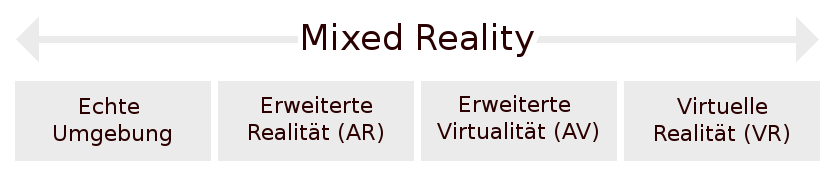
\includegraphics[width=\linewidth]{./img/Mixed_Reality.png}
                \caption{Bestandteile der Mixed Reality \label{fig:MRPic}}
            \end{figure}
            \newline Im Gegensatz zur virtuellen Realität geht es bei der erweiterten Realität darum, dem Nutzer zusätzlich zur wahrgenommenen Realität ergänzende 
            Zusatzinformationen zur Verfügung zu stellen.
            Angefangen wurde mit ersten AR-Anwendungen im Sport: Live-Videos wurden durch Computergrafiken und -animationen erweitert. 
            Bewegte Linien wurden bei bestimmten Bewegungsabläufen eingeblendet. So können beispielsweise Laufwege von Fußballspielern verdeutlicht werden.
            \newline Neuere Entwicklungen befassen sich mit der Mobilkommunikation und unterstützen die Benutzer durch Zusatzinformationen beispielsweise bei der Navigation.
            Für dieses Beispiel sind die Programme darauf ausgelegt, dass der Benutzer die Kamera des Smartphones auf den Straßenverkehr richtet, dem Benutzer wird 
            dann auf dem Display des mobilen Geräts ein Navigationssystem angezeigt. Die Darstellung wird durch Bilderkennung und Ortung des mobilen Geräts ermöglicht.
            Andere Anwendungsmöglichkeiten, als mit einem mobilen Gerät, finden sich bei der Verwendung eines Head-mounted-Displays, wie beispielsweise die Microsoft 
            Hololens.\newline
            Head-mounted-Displays werden umgangssprachlich auch AR-Brillen genannt, da sie dem Nutzer auf den Kopf gesetzt werden und dieser dann durch ein Display 
            schaut. Je nach Programm werden dem Nutzer darauf hin Zusatzinformationen über das Display eingeblendet. Diese Technik findet in Flugsimulatoren oder in der 
            Automotive-Technik statt, beispielsweise zur Schulung von Mitarbeitern.  [AR]
        \section{3D-Audio}
            Aktuelle Surround-Systeme bieten eine gute Klangerfahrung, allerdings fehlen diesen einige Elemente, um eine Erfahrung wie bei einem Live-Konzert zu bieten.  [AudioLabs]\newline
            3D-Audio stellt eine Wiedergabetechnik dar, die realistischer wirkende Audio-Erfahrungen bieten kann als konventionelle 5.1 oder 7.1 Surround-Systeme.
            Die Lautsprecher sind im Gegensatz zu konventionellen Systemen in 3 verschiedenen Ebenen der Höhe angeordnet und umschließen den Nutzer, der sich im optimalen Fall genau mittig des Systems befindet.
            In diesem Projekt werden Audioquellen der Szene hinzugefügt und können um den Nutzer, der sich innerhalb des 3D-Audiosystems befindet, frei bewegt werden. In Verbindung mit der Microsoft 
            HoloLens wird dem Nutzer somit eine Erfahrung geboten, die Audioquelle zu sehen und das sichtbare Audio-Objekt frei um sich herum zu positionieren.       
        \label{sec:2.2}
   
        \section{Verwendete Hard- und Software}
        \label{sec:2.3}
            \subsection{Audio}
            \label{sec:2.3.1Audio}
                \subsubsection{Lautsprechersystem an der HSEL}
                    Um 3D-Audio wiedergeben zu können, wird eine spezielle Lautsprecheranordnung benötigt. Die Hochschule Emden/Leer (HSEL) besitzt ein 
                    22.2 Lautsprechersystem (Abb. 3.1), dass für dieses Projekt genutzt worden ist. Es entstand im Rahmen einer studentischen Projektarbeit und entspricht 
                    der Norm ITU-R BS.2159-7 von der International Telecommunication Union für ein 22.2 Lautsprecher-System.
                    Bedient wird das System von einem Computer inmitten des Lautsprecher-Systems, welcher über Reaper die einzelnen Lautsprecher ansprechen kann.
                    \begin{figure}[htbp]
                        \centering
                        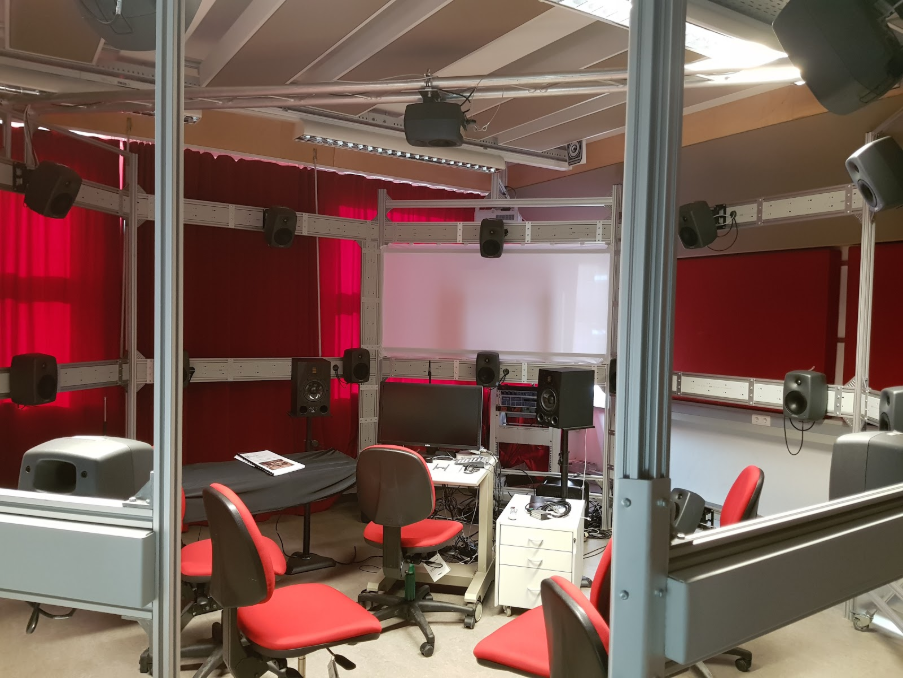
\includegraphics[height=9cm]{./img/Studio.png}
                        \caption{3D-Audio-Labor an der HSEL (Stand: 01/2020)\label{fig:MR}}
                    \end{figure}
                \subsubsection{Reaper}
                \label{sec:3.1.2}
                    Reaper ist eine digitale Audio-Produktions-Applikation, welche unter Anderem für Midi-Aufnahmen, Editierung, Verarbeitung, Mixing and Mastering 
                    genutzt wird. [Reaper]\newline 
                    Reaper kann durch die Unterstützung vieler Plugins und Hardware erweitert werden und wird im Audiolabor zur Ansteuerung des Lautsprechersystems genutzt.
                    Das Projekt nutzt Reaper version 5.985, zur Zeit der Anfertigung dieser Dokumentation ist Reaper 6.02 bereits nutzbar. Anders als bei anderen 
                    Softwarekomponenten in diesem Projekt ist die Version, in der Reaper genutzt wird, nicht ausschlaggebend.                
                \subsubsection{IEM Plug-in Suite}
                \label{sec:3.1.3}
                    Die IEM Plug-in Suite ist eine Open-Source audio plugin suite, welche Ambisonic plugins bis zur 7. Ordnung enthält, erstellt und gewartet vom Institute of 
                    Electronic Music and Acoustics. [IEM]\newline
                    Das Projekt nutzt die IEM Plug-in Suite 1.11.0 vom 15.November 2019. Diese Version ist essentiell für das Projekt, da in Version 1.11.0 jedes 
                    Plugin die Möglichkeit erhalten hat, via OSC informationen zu senden. Zur optimalen Nutzung der erstellten Applikation ist es notwendig, mindestens 
                    die IEM Plug-in Suite 1.11.0 zu installieren.                
                \subsubsection{IEM-MultiEncoder}
                    Mit dem MultiEncoder können mehrere Quellen in einem Plugin encodiert werden. Dazu kann der Nutzer oben links im Plugin die gewünschte 
                    Anzahl der Quellen wählen und diese dann nach eigenen Wünschen unter den Encoder settings im jeweiligen Azimuth, Elevation und Gain ändern. 
                    Ebenso hat der Nutzer die Möglichkeit, jede Quelle zu muten, solo auszuwählen, oder auch die ganze Kugelhülle zu bewegen.
                    Ebenso ist es möglich, wie mit allen Plugins der IEM Plug-in Suite, OSC-Nachrichten zu senden und zu empfangen.
                    \begin{figure}[htbp]
                        \centering
                        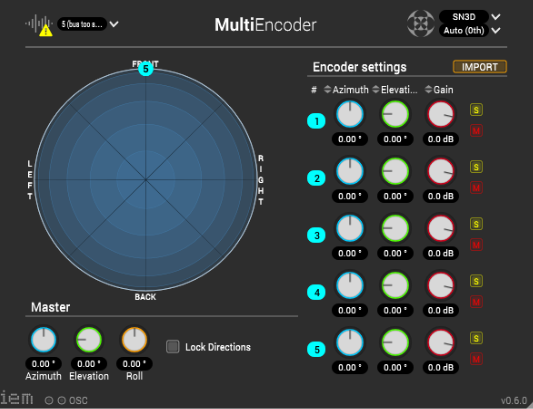
\includegraphics[height=6cm]{./img/MultiEncoder.png}
                        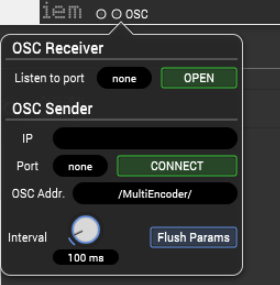
\includegraphics[height=6cm]{./img/MultiEncoderOSC.png}
                        \caption{Bedienoberfläche des IEM MultiEncoders \label{fig:MultiEncoder}}
                    \end{figure}
                    \subsection{Video}
            \label{sec:2.3.2Video}
                \subsubsection{HoloLens}
                    Die Microsoft HoloLens ist eine Mixed-Reality Brille, durch die der Nutzer interaktive 3D-Projektionen in der Umgebung darstellen kann.
                    [HoloLens]\newline
                    Die HoloLens kommt - anders als viele Mitbewerber - ohne zusätzlichen Computer oder Smartphone aus.
                    Als Betriebssystem dient das Microsoft-eigene Windows 10, allerdings eine auf Mixed-Reality-Anwendungen zugeschnittene Version.
                    Die HoloLens verfügt über mehrere Sensoren, eine Kamera und zwei Lautsprecher.
                    Über die Sensoren und die Kamera werden kann die Brille Handgesten des Nutzers deuten und die räumlichen Gegebenheiten analysieren.
                    2019 stellte Microsoft die weiterentwickelte HoloLens 2 vor. Diese wird seit November 2019 ausgeliefert, leidet aber zur Zeit 
                    (stand: Januar 2020) noch immer unter Lieferschwierigkeiten durch eine hohe Nachfrage [Mixed]. Die Hololens 2 zeichnet sich durch 
                    ein größeres Display, Erkennung von Fingern und einem höheren Tragekomfort aus.
                    Zur Bedienung der HoloLens sind Gesten notwendig. [Abb. Gestures]
                    \begin{figure}[htbp]
                        \centering
                        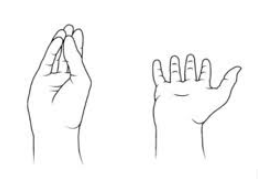
\includegraphics[height=4cm]{./img/Gesture1.png}
                        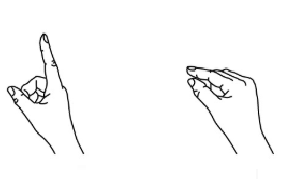
\includegraphics[height=4cm]{./img/Gesture2.png}
                        \caption{Geste "Blume" zum Öffnen des Menüs (links) und "Tap" zum Bestätigen oder Greifen (rechts) \label{fig:Gestures}}
                    \end{figure}
                \subsubsection{Mixed Reality Toolkit}
                    Das Mixed Reality Toolkit ist eine von Microsoft erstellte Sammlung von Software-Komponenten, um möglichst schnell und einfach 
                    Mixed-Reality (AR und VR) Applikationen zu erstellen. [MRTK]\newline
                    Das MRTK ist nutzbar zur Entwicklung für die Microsoft HoloLens, die Microsoft HoloLens 2, Windows Mixed Reality headsets und OpenVR 
                    headsets wie die HTC Vive oder Oculus Rift.
                    Für dieses Projekt wird Version 2.0.0 genutzt. Ältere Versionen sind mit diesem Projekt wahrscheinlich nicht kompatibel, 
                    auch neuere Versionen (aktuell neuste Version: 2.1.0) können Änderungen enthalten, die nicht abwärtskompatibel sind und 
                    somit eine Umstrukturierung des Projekt nötig ist.\newline
                    Das MRTK hilft den Entwicklern bei der Erstellung von Komponenten, die in jeder Mixed Reality Applikation benötigt werden, 
                    wie beispielsweise Buttons oder Verhaltensweisen von Objekten bei deren Berührung. Dazu werden die zur Verfügung stehenden Skripte
                     seitens Microsoft einfach den gewünschten Objekten in der Szene hinzugefügt und nach den Bedürfnissen des Entwicklers angepasst.
                
                \subsubsection{Unity}
                    Unity ist eine Laufzeit- und Entwicklungsumgebung für Spiele des Unternehmens Unity Technologies. Mit Unity können 2D- und 
                    3D-Applikationen für Windows, Linux, Mac und gängige Spielekonsolen erstellt werden [Unity-Spiel-Engine] und ist neben der 
                    Unreal Engine, Frostbite und CryEngine eine der am häufigsten verwendeten Spiele-Engines. [Spiel-Engine]\newline
                    Allerdings ist Unity nicht nur für Spiele geeignet, sondern kann auch für Film und Animation, oder auch für Mixed Reality 
                    Anwendungen genutzt werden. [unity]\newline
                    Die Entwicklungsumgebung Unity ist einer herkömmlichen Animationssoftware ähnlich aufgebaut. Das Hauptfenster stellt eine Szene dar,
                    der sogenannte “GameObjects” hinzugefügt werden. Den GameObjects können Komponenten (Materialien, Klänge, physikalische Eigenschaften, 
                    Code-Skripte) zugefügt werden, durch die die Szene individuell gestaltet werden kann.\newline
                    Das Projekt verwendet Unity in der Version 2019.2.2f1. Diese Version ist essentiell zur Verwendung des Projekts. Unity hat einen 
                    Aktualisierungszyklus von ungefähr zwei Wochen für eine neue Version, allerdings ist es gegebenenfalls nötig alle Assets neu 
                    zu importieren, sofern der Entwickler die Unity-Version aktualisiert.
            \subsection{Datenübertragung}
            \label{sec:2.3.3Daten}
                Open Sound Control ist ein Kommunikationsprotokoll zwischen Computern, Synthesizern und anderen Multimedia-Geräten zur Kommunikation 
                zwischen den Geräten über ein Netzwerk. [OSC]\newline
                OSC ist der Standard zur Übertragung von Audio-basierten Daten und wird von den gängigen DAWs unterstützt. 
                Dieses Projekt verwendet OSC zur Übertragung von Daten zwischen der DAW Reaper und der HoloLens. Um OSC in Unity zu verwenden, 
                wird die Software OSC simpl (for Unity) verwendet.
                \subsubsection{OSC Simpl}
                OSC simpl ist ein Unity Asset Store Produkt der dänischen interaction design consultancy Sixth Sensor [Sixth Sensor]. 
                OSC simpl ist die vorgeschlagene Implementation von opensoundcontrol.org und im Unity Asset Store käuflich erwerblich. [osc simpl]
                OSC simpl macht es dem Entwickler leicht, OSC Nachrichten zu senden und zu empfangen. Dazu erhält ein leeres GameObject zwei Skripte 
                von OSC simpl, eins zum empfangen und eins zum senden. Im Unity-Inspector müssen nur noch die Ip-Adresse und der Port des 
                Empfängers eingegeben werden, dann können Daten ausgetauscht werden. 
                    
            \subsection{Versionskontrolle}
            \label{sec:2.3.4Kontrolle}
                \subsubsection{Git}
                    Git ist ein freies verteiltes Versionsverwaltungssystem, entwickelt unter Anderem vom Linux Gründer Linus Torvalds. [Git]
                    In der Softwareentwicklung ist die Versionsverwaltung in Projekten mit mehreren Entwicklern essentiell um Konflikte bei Änderungen 
                    von Textdateien, wie etwa Quelltexten, zu vermeiden und wird aus selbigen Gründen in diesem Projekt genutzt.
                    Git unterscheidet sich von anderen Versionsverwaltungssystemen unter Anderem durch eine Nicht-lineare Entwicklung, dem Fehlen eines 
                    zentralen Servers, kryptographischer Sicherheit der Projektgeschichte und vielen weiteren Funktionen.
                \subsubsection{Github}
                    Github ist ein Onlinedienst zur Bereitstellung von Software- Entwicklungsprojekten. [Github] Seit Dezember 2018 gehört das 
                    Unternehmen zu Microsoft. Github macht es dem Nutzer sehr einfach, an vielen Quelltext-Datenbanken - den sogenannten 
                    Repositories - mitzuwirken, in dem ein Buttonklick genügt, um eine Abspaltung eines fremden Repositories zu erhalten 
                    (die sogenannte “fork”).
                    Dieses Projekt hat eine zentrale Hauptprojekt-stelle, alle anderen Entwickler haben eine Fork dieses Projekts vorgenommen.
                    Jeder Entwickler kann so in einem eigenen Projekt arbeiten.
                    Nachdem ein Entwickler eine neue Funktion dem Hauptprogramm zur Verfügung stellen will, kann ein sogenannter “Pull-Request” 
                    an das Hauptprojekt gestellt werden. Der Besitzer des Hauptprojekts kann daraufhin die vorgenommenen Änderungen des Fremdentwicklers 
                    prüfen und entscheiden, ob diese in das Hauptprojekt übernommen werden sollen.
    \chapter{Praxis}% Kapitel 3
    \label{sec:Praxis}                
        \section{Aufgabenstellung der Arbeit}
        \label{sec:3.1}
            \subsection*{Zielsetzung}
                Das Ziel dieser Arbeit ist die Visualisierung aller im MultiEncoder verfügbaren Elemente in einer virtuellen 
                Umgebung unter Nutzung der HoloLens. Auf die bereits zu Beginn des Projekts verfügbare Funktion, eine einseitige 
                Verbindung von Unity zu REAPER herzustellen, soll aufgebaut werden.
            \subsection*{Ausgangssituation des Projektes}
                Die ursprüngliche Intention des Projekts lag in der Visualisierung der Elemente des Multiencoders mittels einer 
                virtuellen Umgebung in Unity unter Nutzung der HoloLens. Dabei war es zum Ausgangspunkt des Projekts bereits 
                möglich mittels des OSC Send Scripts eine Verbindung zwischen REAPER und Unity herzustellen. Über diese 
                Verbindungen war es möglich, einseitig die Position einer Kugel an REAPER zu senden und den Kanalparametern 
                Azimuth und Elevation zuzuordnen. Dabei war die korrekte Berechnung der jeweiligen Parametern noch fehlerhaft. 
                Des Weiteren war die Anzahl der verwendeten Kugeln noch nicht den Kanälen entsprechend dynamisch sondern musste 
                manuell über Unity eingestellt werden. Zusätzlich zu Azimuth und Elevation sollten auch andere Kanal relevante 
                Parameter wie der Gain oder die Kanalanzahl implementiert werden.
            \subsection*{Synchrone Kommunikation der Umgebungen}
                Um einen beidseitigen Austausch zwischen Unity und Reaper zu ermöglichen muss neben dem OSC Send auch das OSC Input 
                Script implementiert werden um dadurch den Empfangsweg von Reaper zu Unity zu ermöglichen und beispielshalber eine 
                Änderung der Kanalparameter von seiten Reapers in eine Positionsveränderung in Unity zu übertragen.\newline	
                Damit die Anwendung effektiv auf der HoloLens eingesetzt werden kann, muss dafür gesorgt werden, dass Reaper und die 
                HoloLens synchron arbeiten. Wird beispielshalber mit der HoloLens eine Kugel in der Anwendung bewegt, sollte dies in 
                Echtzeit in einer Parameteränderung in Reaper resultieren und umgekehrt ebenso abgebildet werden.
            \subsection*{Vereinfachung der Bedienung TOD}%TODO
                Neben den oben genannten Parametern gilt es die Anwendung um zwei weitere wichtige Aspekte zu erweitern. Dieser ist zum 
                einen die Kanalanzahl, durch welche der Benutzer in Reaper seinem Projekt weitere Tonspuren hinzufügen kann um diese 
                dann durch die korrespondierenden Kugeln in Unity beliebig im Raum zu verteilen. Dabei sollte die Kanalanzahl 
                beidseitig, also auf seiten Reapers sowie in der VR Anwendung, einstellbar sein und stets mit der Anzahl der Kugeln 
                in der VR Anwendung übereinstimmen.
                Der zweite Aspekt ist der Audioparameter Gain. Dieser steuert auf seiten REAPERs die Eingangslautstärke der jeweiligen 
                Tonspur. Eine Implementierung in die VR Anwendung würde bedeuten, dass dieser Parameter ebenfalls über die Interaktion 
                mit der Sphere für den jeweiligen Kanal verändert werden kann und infolgedessen wie die Kanalanzahl zwischen beiden 
                Programmen synchronisiert werden muss.
            \subsection*{Optimierung des Entwicklungsprozesses}
                Zusätzlich soll eine Entwicklungsumgebung in Form einer dedizierten Entwicklungsszene in Unity geschaffen werden, 
                welche den Entwicklungs- und Testprozess innerhalb oder im Anschluss an dieses Projekt weitestgehend beschleunigen 
                soll. Dies soll alle für den Entwicklungsprozess wichtigen Einstellungen vom Unity Benutzerinterface in die 
                jeweilige Szene oder Anwendung verlagern um den Prozess dadurch für den Anwender zu zentralisieren und zu 
                vereinfachen.
        \newpage
        \section{Ergebnisse}
            Im folgenden Kapitel wird der aktuelle Stand des Projektes näher erläutert. Dabei wird verstärkt Augenmerk auf die 
            Systemstruktur, OSC Verbindung, Kommunikationswege und Parameterberechnung gelegt.
        \label{sec:3.2}
            \subsection{Systemarchitektur gemäß C4-Modell}
            \label{sec:3.3.1}
                Das Softwaresystem, das durch diese Projektarbeit geschaffen worden ist, ist nicht in einem einfachen standard 
                UML-Diagramm auszudrücken, da unterschiedliche Abstraktionen (Schnittstelle Reaper -> HoloLens, OscSimpl Asset, MRTK,...) 
                zu beachten sind, die in sich geschlossene Softwaresysteme darstellen. Aus diesem Anlass wird die System-Architektur 
                folgend nach dem C4 Modell [C4model] dargestellt. Durch dieses Modell kann das Komplettsystem in seine Teilsysteme 
                anschaulich heruntergebrochen werden. 
                Da das C4 Modell noch kein UML-Standard ist, eine kurze Erläuterung der Abstraktionen: 
                An oberster Stelle steht die Person, die das Software-System nutzt. Dies kann ein Endnutzer, oder auch ein anderer Nutzer 
                mit bestimmten Rollen sein.
                Darunter folgt die höchste Abstraktionsschicht, ein Software-System. Software-Systeme sind abgeschlossene Applikationen, 
                deren Zusammenspiel im System-Context veranschaulicht werden.
                Ein System-Context kann mehrere Container enthalten. Container sind Sammlungen von Applikationen, die zur Nutzung des 
                Systems notwendig sind, aber unabhängig voneinander bestehen können, wie beispielsweise eine Web-Applikation und eine 
                Datenbank-Anbindung.
                Container wiederum enthalten Komponenten. Komponenten lassen sich als Gruppierung von zugehörigen Funktionalitäten 
                verstehen. In Kontext um Unity werden Komponenten mit GameObjects gleichgesetzt, da GameObjects mehrere zusammengehörige 
                Skripte besitzen.
                \begin{figure}[htbp]
                    \centering
                    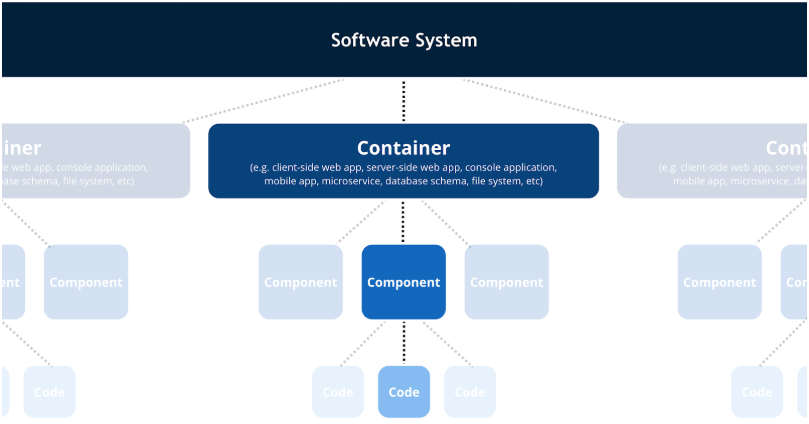
\includegraphics[width=14cm]{./img/c4Model.png}
                    \caption{Das C4 Modell visualisiert ein Komplettsystem durch die Aufgliederung in Teilsysteme.\label{fig:C4}}
                \end{figure}

                \subsubsection*{System Context}
                    Die oberste Position im C4 Modell auf dieses Projekt bezogen wird durch den Anwender belegt, also zum Beispiel einem 
                    Tonmeister. Dieser kann die Audioquellen via Reaper (MultiEncoder) oder HoloLens-Applikation beeinflussen. 
                    Änderungen an einer der beiden Softwaresysteme werden mit der jeweils anderen synchronisiert (Abb. 1337).
                    \begin{figure}[htbp]
                        \centering
                        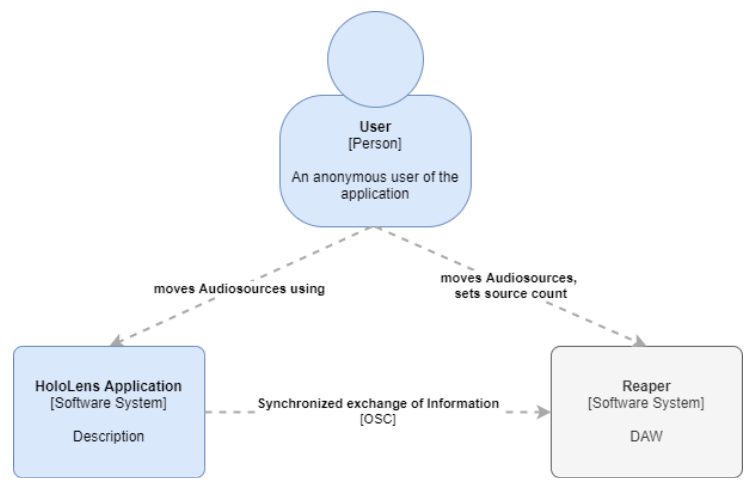
\includegraphics[width=14cm]{./img/systemContext.png}
                        \caption{Unabhängig vom Ort der Befehlseingabe synchronisieren sich die Systeme.\label{fig:systemContext}}
                    \end{figure}
                \subsubsection*{Container}
                    Die mit diesem Projekt entwickelte HoloLens-Applikation basiert auf zwei Softwarepaketen. Zum Einen auf dem MRTK für 
                    den Inhalt der Szene in Unity (siehe 3.1.2), zum Anderen auf OSCSimpl für die Kommunikation im Netzwerk (siehe 3.1.3). 
                    Beide Container setzen sich wiederum aus mehreren Komponenten zusammen.
                    \begin{figure}[htbp]
                        \centering
                        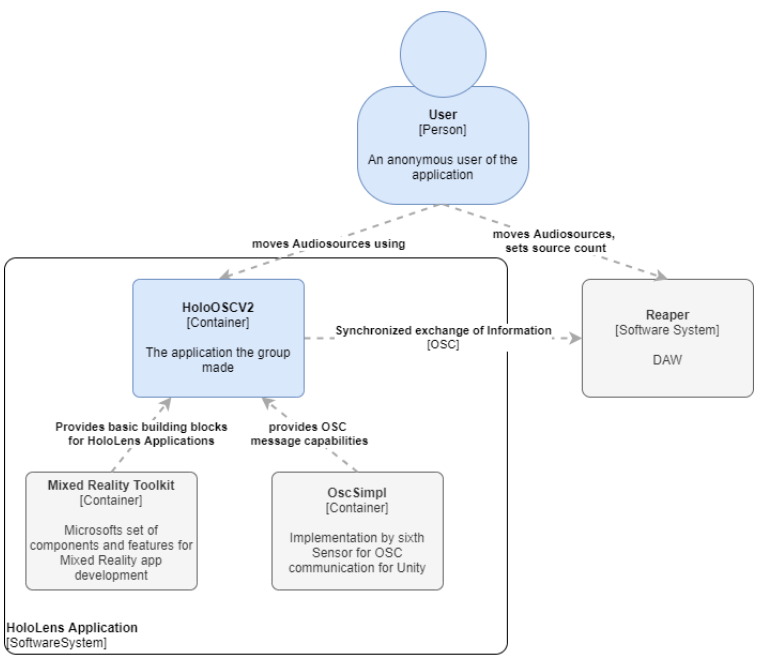
\includegraphics[width=14cm]{./img/container.png}
                        \caption{Das Zusammenspiel von MRTK und OSCSimpl als Grundlage der Applikation. \label{fig:containerPic}}
                    \end{figure}
                \subsubsection*{Component}
                    Die Szene der AR-Applikation besteht aus mehreren Objekten. Der Anwender selbst befindet sich in einer 
                    Gitternetzkugel (“Shell”). Diese stellt die Ausdehnung des Lautsprecher-Arrangements dar. Sichtbar sind weiterhin 
                    die im Multiencoder eingestellten Kanäle in Form von kleineren Kugeln (“Sources”) auf der Hülle der Gitternetzkugel 
                    sowie eine Benutzeroberfläche mit Schaltflächen und Verbindungsanzeige. In der Szene ebenfalls vorhanden, jedoch 
                    für den Anwender nicht sichtbar sind der SourceHandler und der OSC Handler.
                    Dies sind die Komponenten der oben genannten Container. Diese Objekte sind weiterhin ebenfalls mit mehreren Skripten 
                    belegt, deren Funktionen sich in Parameterberechnungen und Nachrichtenverarbeitung spezialisieren. 
                    \begin{figure}[htbp]
                        \centering
                        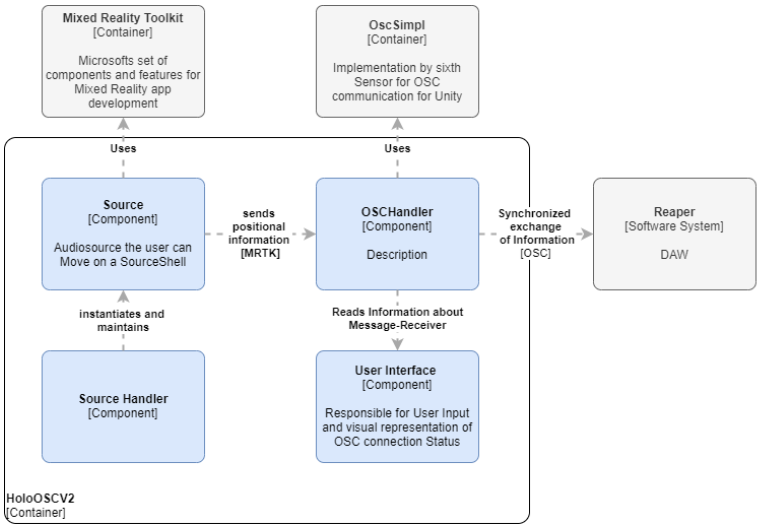
\includegraphics[width=14cm]{./img/component.png}
                        \caption{Unity-Objekte der AR-Anwendung (blau hinterlegt) als Komponenten übergeordneter Softwarepakete zur Koordination von Informationen.\label{fig:container}}
                    \end{figure}
            \subsection{OSC-Verbindung zwischen Unity und IEM MultiEncoder}
            \label{sec:3.2.2}
            Wie im letzten Kapitel beschrieben, sind SourceHandler und OSC Handler unsichtbare Objekte in der Szene. 
            Für den Verbindungsaufbau ist der OSC Handler verantwortlich. Dieser besteht aus fünf Skripten, deren Zusammenwirken 
            außerdem das Empfangen, Verteilen und Versenden von Nachrichten ermöglicht. 
                \subsubsection{Darstellung der Kommunikation via OSC}
                    Die folgenden zwei Abbildungen zeigen schematisch die Verbindungen der einzelnen Elemente. Skripte des OSC-Handlers 
                    sind grün hinterlegt und werden anschließend erläutert.
                    \begin{figure}[htbp]
                        \centering
                        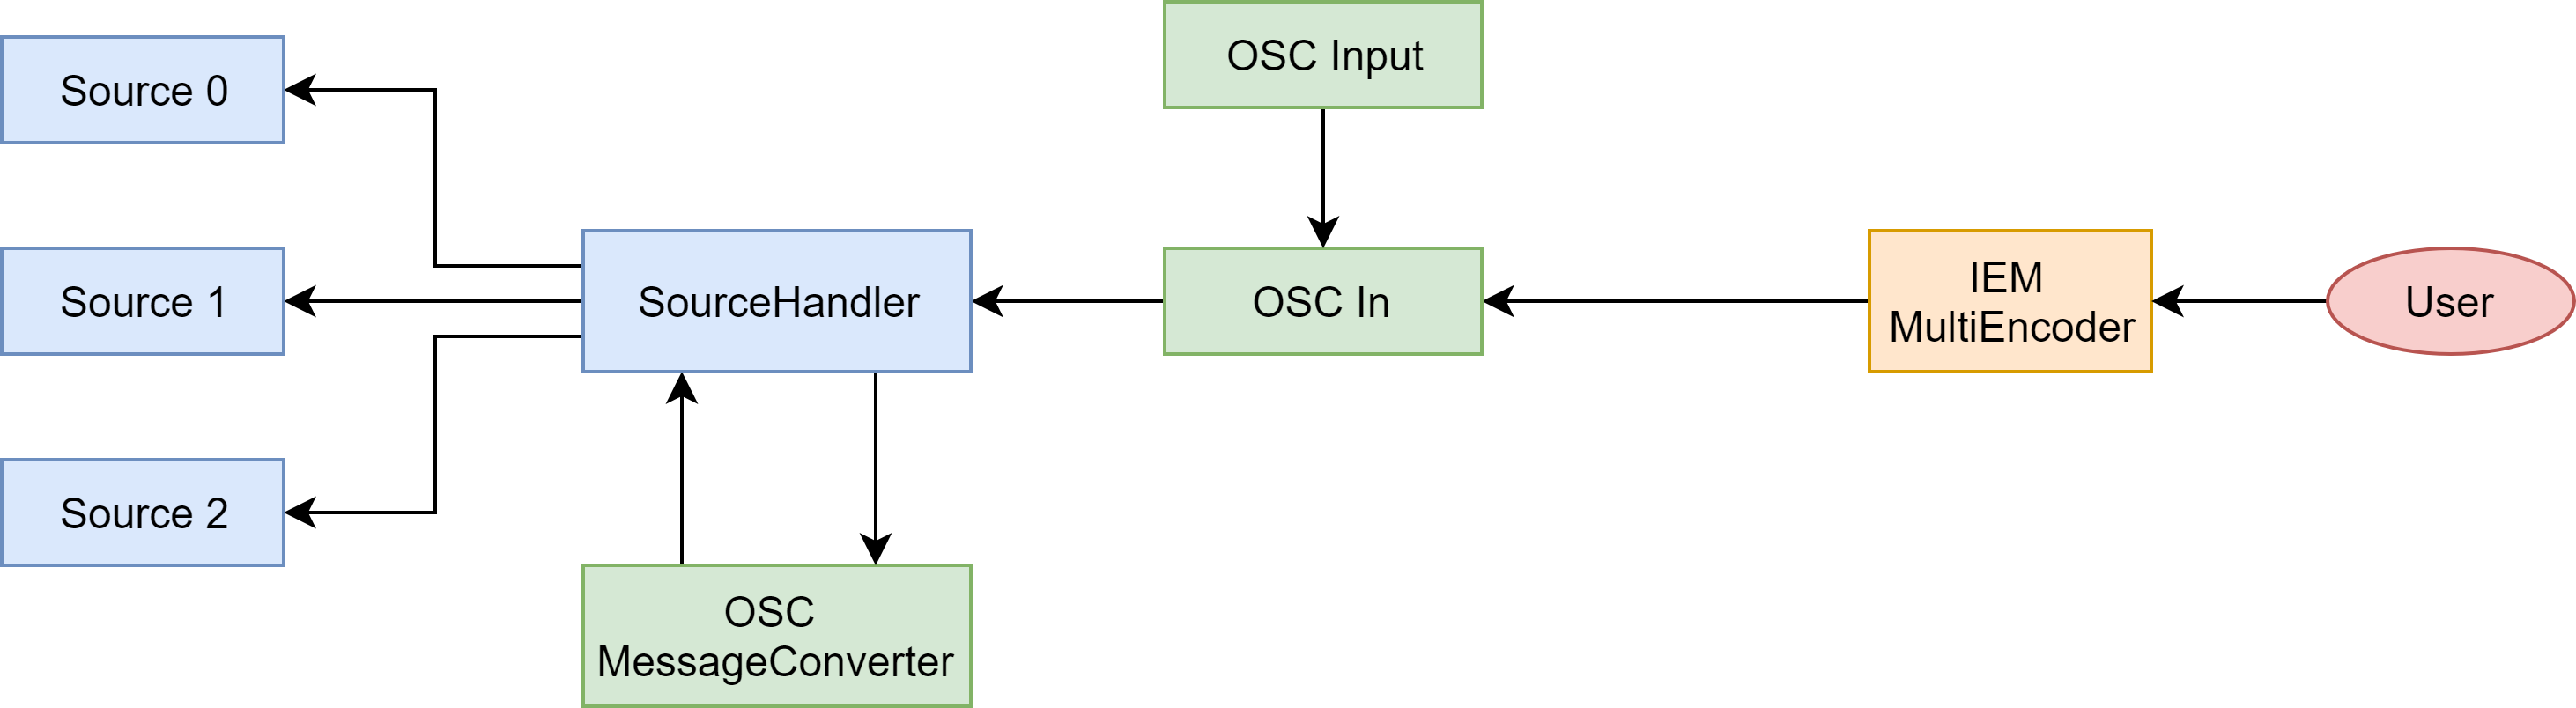
\includegraphics[width=\linewidth]{./img/eingehend.png}
                        \caption{Darstellung der Verarbeitung eingehender OSC-Nachrichten.\label{fig:in}}
                    \end{figure}
                    \begin{figure}[htbp]
                        \centering
                        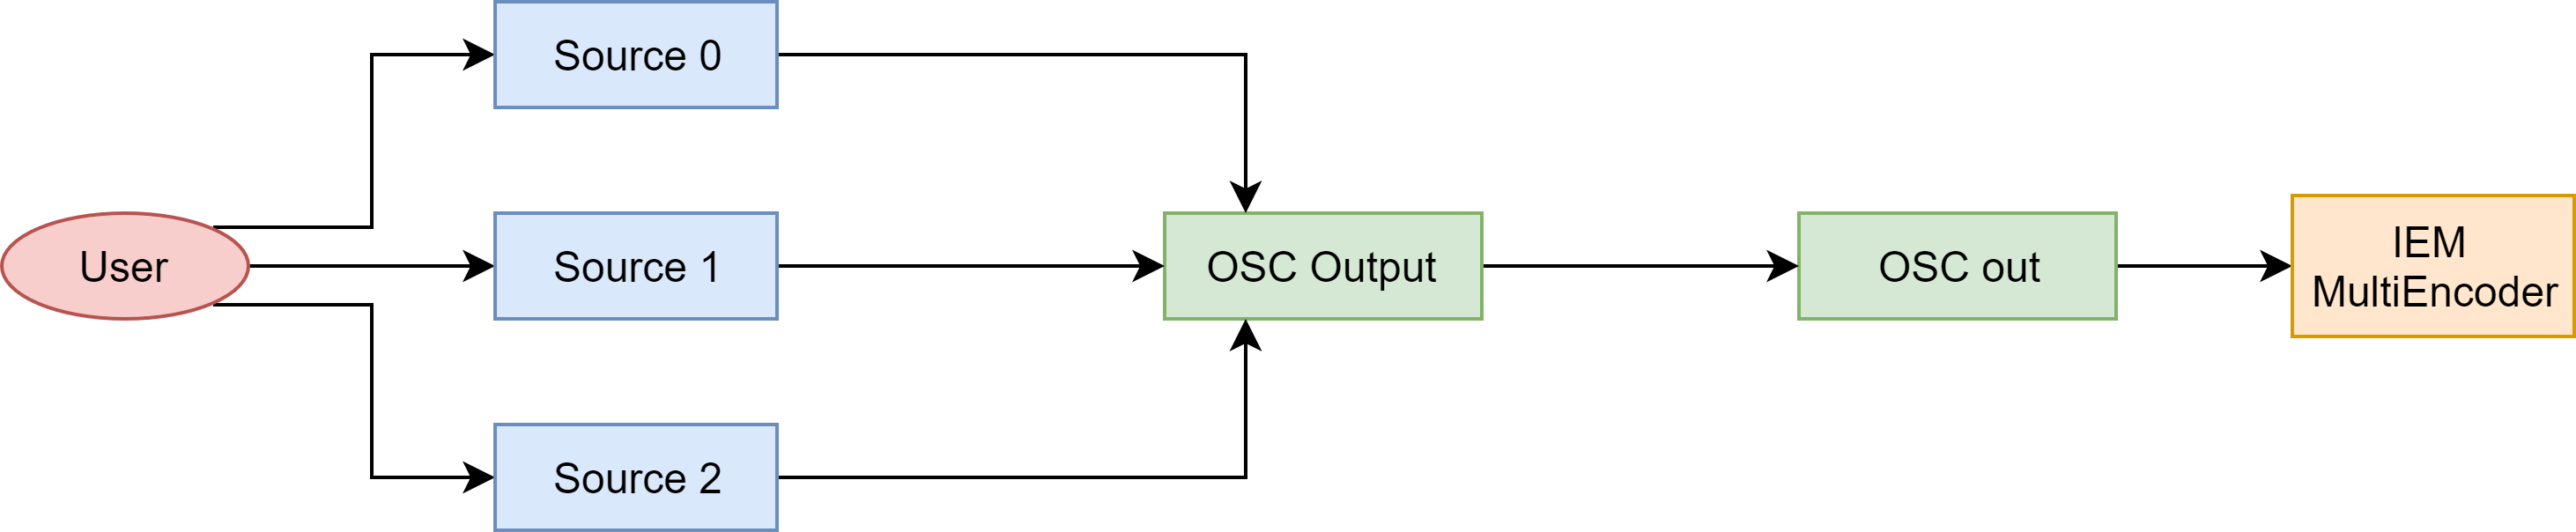
\includegraphics[width=\linewidth]{./img/ausgehend.png}
                        \caption{Darstellung der Verarbeitung ausgehender Nachrichten.\label{fig:out}}
                    \end{figure}
                \subsubsection{Der OSC-Handler}
                    \paragraph{Skript - OSC Out}
                    Dieses Skript ist Teil des Assets OSC Simpl und bietet Methoden zum Senden von OSC Nachrichten. 
                    In dieser Anwendung  also die Parameter der einzelnen Kanäle für den MultiEncoder in Reaper. 
                    Gameobjects mit diesem Skript sind OSC Clients. Daher benötigt es die IP Adresse und Port des 
                    Empfängers, in diesem Falle also des Rechners auf dem Reaper läuft. Es können weitere Einstellungen 
                    zur Art und Weise des Sendens vorgenommen werden, die hier nicht weiter genannt werden.
                    Ist der OSC Handler in Unity ausgewählt, so werden im Inspector bei diesem Skript in einem 
                    Nachrichtenfenster alle ausgehenden Nachrichten aufgelistet.
                    \paragraph{Skript - OSC Output} 
                    Um Eingaben der Hololens für die Netzwerkverbindung korrekt auszuwerten, wird dieses Skript benötigt. 
                    Es beinhaltet Methoden zur Initiierung des Verbindungsaufbaus- und Aktualisierung. Diese werden über 
                    Schaltflächen in der Szene gesteuert. Die in der Anwendung eingegebene IP und Port werden durch den 
                    ReceiverAdressConverter umgewandelt, sodass OSC Out benutzt werden kann.
                    \paragraph{Skript - OSC In TOOOOOODOOOOOOOO}     
                    Auch dieses Skript ist Teil von  OSC Simpl und bietet Methoden zum Empfangen von OSC Nachrichten. 
                    Gameobjects mit diesem Skript sind OSC Server. Um den OSC Server zu starten, muss lediglich ein 
                    Port geöffnet werden. Dieser muss den entsprechenden Angaben im MultiEncoder unter OSC Sender 
                    gleichen (siehe Abb. 3.2). Eingehende Nachrichten werden mit einer Map in für Unity nutzbaren Code umgewandelt. 
                    Auch hier befindet sich sichtbar auf dem OSC Handler ein Nachrichtenfenster in dem alle eingehenden 
                    Informationen gelistet sind.
                    \paragraph{Skript - OSC Input}
                    Dieses Skript öffnet den Port zum Empfangen von Nachrichten und erstellt Maps für OSC In. Dadurch werden 
                    Informationen von OSC In angepasst und an den SourceHandler übergeben.
                    \paragraph{Skript - OSC Message Converter}
                    Damit der SourceHandler die eingegangenen Nachrichten auswerten kann um die richtigen Werte an die 
                    entsprechende Source weiterzuleiten, wird dieses Skript benötigt. Es zerlegt jede Nachricht in Adresse, 
                    Kanalnummer, Parameter und Wert.
                \subsubsection{OSC im Multiencoder}
                    In der hier verwendeten Version (siehe 3.1.1) sind im MultiEncoder lediglich die Ports bzw. IP Adressen des 
                    Ein- und Ausgangs festlegbar. Es kann zusätzlich der in der Adresse vorkommende Name vorgegeben werden. 
                    Das Sendeverhalten an sich jedoch, kann nicht beeinflusst werden. Bei Änderung eines Wertes auf einem der 
                    Kanäle wird genau nur diese Änderung als Nachricht verschickt. Auf Knopfdruck “Flush Params” (vergl. Abb 3.2) sendet der MultiEncoder 
                    alle Werte von allen Kanälen nacheinander. Bei vierundsechzig Kanälen mit je drei Werten werden entsprechend knapp 
                    zweihundert Nachrichten verschickt, auch wenn nur ein Kanal aktiv ist. Eine direkte Abfrage von Werten ist nach 
                    aktuellem Stand nicht möglich
                \subsubsection{Connection Status}
                    Die Verbindungsanzeige befindet sich äußerst rechts im User Interface und signalisiert dem Benutzer den aktuellen Verbindungsstatus. 
                    Da es bisher keine Möglichkeit gibt ohne Änderung eines Wertes Informationen vom MultiEncoder zu bekommen, besteht die 
                    Verbindungsabfrage aktuell aus der Benutzung des letzten Kanals. Regelmäßig wechselndes Stummschalten des Kanals dient 
                    hier als provisorischer Ping.
                    \begin{figure}[htbp]
                        \centering
                        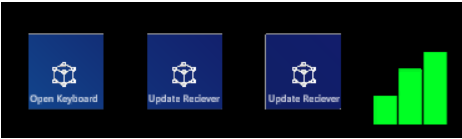
\includegraphics[width=7cm]{./img/status.png}
                        \caption{ Aktueller Screenshot der Benutzeroberfläche, äußerst rechts die Verbindungsanzeige.
                        \label{fig:status}}
                    \end{figure}
            \newpage 
            \subsection{Berechnung und Auswertung der Parameter}
            \label{sec:3.2.3}
                Die Szene, in der sich der Nutzer mit der Hololens bewegt besteht aus einer SourceShell, die das Gestell der 
                Lautsprecherarrangierung im 3D-Labor darstellt (hier eine Gitterneztkugel), sowie aus kleineren Kugeln, die die 
                Schallquellen bzw. Kanäle des MultiEncoders darstellen. Diese Kugeln bewegen sich ausschließlich auf der Hülle der 
                SourceShell deren Zentrum durch die Position im Raum der Hololens beim Laden der Szene festgelegt wird. Gleiches gilt 
                für die Ausrichtung des globalen Koordinatensystems der Szene.
                \subsubsection{Bestimmung und Festlegung von Azimuth und Elevation}
                    Durch den SourceHandler eingehende Werte für Elevation und Azimuth sind aufgrund der Nachricht vom Multi-Encoder 
                    in Winkel angegeben. Der Radius der Hülle, die den Dimensionen der Lautsprecheranordnung angepasst ist, ist im Code 
                    bereits definiert. Durch zwei Winkel und einem Radius lässt sich die Position im Raum genau beschreiben. 
                    Die betroffene Source wandelt diese mit Hilfe des CoordinateTransformService in Kartesische Koordinaten um und 
                    definiert somit ihre Position in der Szene. Ändert sich jedoch die Position einer Quelle in der Szene durch den Nutzer der Hololens, werden ihre aktuellen 
                    kartesischen Koordinaten in Kugelkoordinaten umgerechnet und an OSC Output gesendet.\newline
                    \begin{wrapfigure}{l}{0.45\textwidth}
                        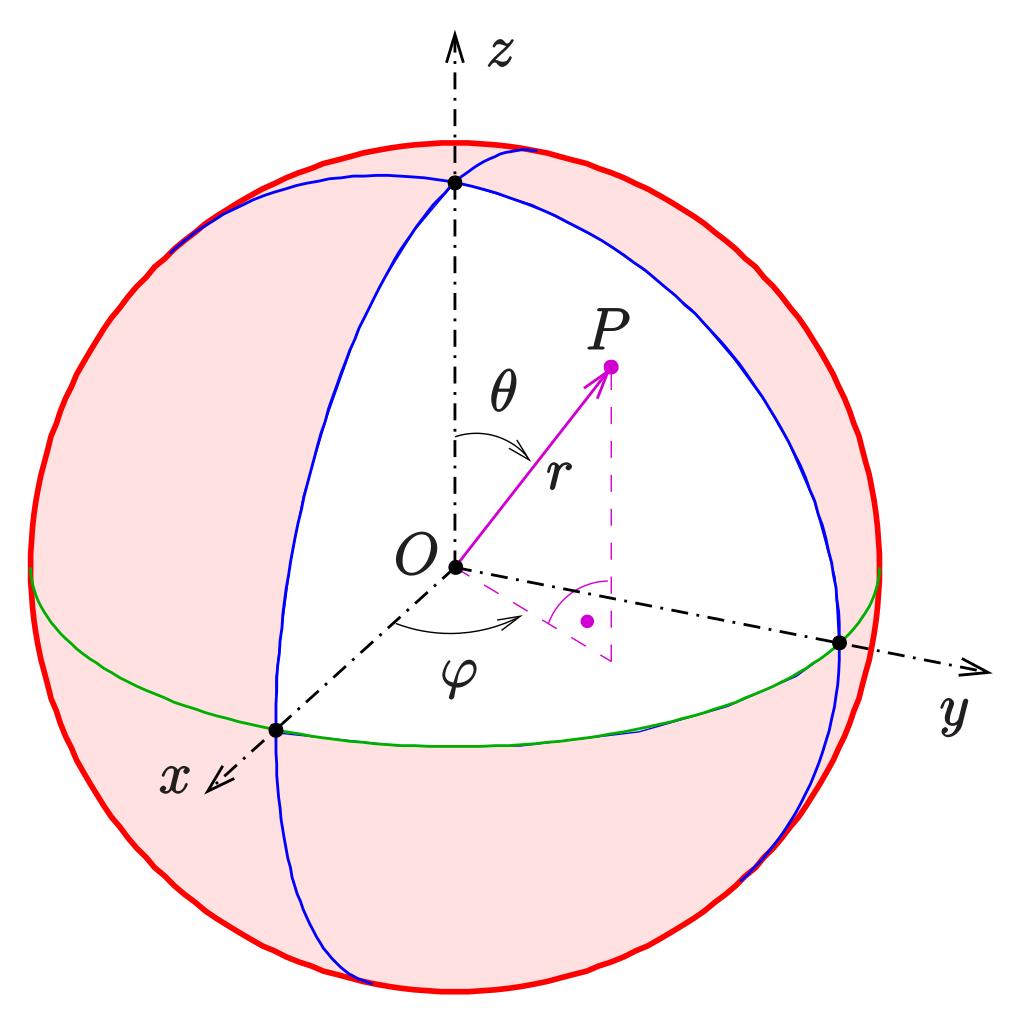
\includegraphics[width=7cm]{./img/kugel.png}
                        \caption{ Darstellung kartesischer und sphärischer Koordinaten.
                        \label{fig:kugel}}
                    \end{wrapfigure}
                    Hier gilt es zu beachten, dass die Koordinaten in Unity anders als auf dem Bild dargestellt, ausgerichtet sind.
                    Die Abbildung repräsentiert daher nicht die folgenden im Code verwendeten Formeln!
                    In Unity ist die Y-Achse vertikal und die horizontale Ebene wird durch die X- und Z-Achse aufgespannt.
                    Der MultiEncoder rechnet mit der Elevation, abgebildet ist jedoch die Inklination.\newline\newline
                    \large 
                    $Px=r*\cos(\Theta)*\sin(-\Phi)$ \newline
                    $Py=r*\sin(\Theta)$ \newline
                    $Pz=r*\cos(\Theta)*\cos(-\Phi)$ \newline\newline
                    \normalsize Elevation:
                    \large $\Theta = \arcsin(\frac{y}{r})$\newline
                    \normalsize Azimuth: 
                    \large $\Phi =-atan2(x,z)$\normalsize\newline
                    \newline\newline\newline
                    
                    \newpage
                \subsubsection{Grafische Darstellung des Lautstärkepegels (Gain)}
                    Die Werte des Gains im MultiEncoder befinden sich zwischen minus sechzig und plus zehn Dezibel. Damit die Szene 
                    übersichtlich und wortwörtlich greifbar für den Anwender bleibt, wird die Dynamik der Größenveränderung stark eingeschränkt. 
                    Auf jeder Source in der Szene befindet sich das Skript “TransformScaleHandler”. Dieses ist Bestandteil des MRTK und dient 
                    der Festlegung eines Minimal- und Maximalwertes zur Skalierung einer Kugel. 
                    Die Umrechnung der Werte übernimmt die Source selbst. Eingehende Werte werden in den positiven Zahlenbereich verschoben, 
                    auf den vorgegebenen Dynamikumfang der Szene normiert und auf den Minimalwert addiert. Ausgehende Werte werden dementsprechend 
                    wieder auf den höheren Dynamikumfang des MultiEncoders skaliert und um sechzig Werte in den negativen Zahlenbereich verschoben. 
                    Durch diese Umrechnung entstehen aufgrund des Verhaltens von Fließkommazahlen minimale Abweichungen, die jedoch gering und 
                    somit nicht weiter zu betrachten sind.\newline
                    Kugeln im Raum, die auf den Minimalwert skaliert sind, haben im MultiEncoder den Wert -60 dB und sind somit stumm. 
                    Daher wechselt ihre Farbe in der Szene um es ebenfalls übersichtlicher für den Anwender zu machen.
            \subsection{Tooltips zur Kanalzuordnung}
            \label{sec:3.3.4}
                Damit der Benutzer innerhalb der Szene erkennen kann welche Kugel zu welchem Kanal gehört, wurden Tooltips implementiert. 
                Das Tooltip-GameObject ist ein Child des Source-GameObject-Prefabs um die Positionen im Raum von Kugel und Tooltip zu verbinden. 
                Da sich alle Sources im SourceHandler in einem Array befinden und die Source-ID gemäß ihrer Position im Array vergeben wird, 
                sind Source-ID und Tooltiptext um eins verschoben. (Source-ID “0” als erste Kugel hat also den Tooltip “1” für Kanal “1”).   
            \subsection{Entwicklungsszene in Unity}%TODO
            \label{sec:3.2.5}
    \chapter{Zusammenfassung}% Kapitel 4
    \label{sec:org12d8e10}
        \section{Ergebnis}
        \label{sec:4.1}
        \section{Diskussion}
        \label{sec:4.2}
        \section{Ausblick}
        \label{sec:4.3}
                    

\end{document}